\chapter{Command mode and assisted mode}\label{ch:modes}

Two more faces, for the same reason the console exists: what a person needs from
the page depends on what they are doing. An analyst who repeats the same report
every week wants to write it down once and run it. An analyst who is deciding what
to include wants to see the choices. Both end at the same place --- a report or an
archive --- and both drive one catalogue, so the two never disagree about what can
be produced.

They sit either side of the console in the status bar, so the three ways of
working are one row apart.

{\small\noindent\makebox[\textwidth][l]{\begin{tabular}{@{}ll@{}}
\toprule \textbf{Button} & \textbf{Opens} \\\midrule
Stop & stops the running task \\
Command mode & command mode \\
Console mode & the console \\
Assisted mode & assisted mode \\
Save status report & writes the status report \\
Details & the detail lines \\
\bottomrule
\end{tabular}}}


\section{One catalogue}
Everything that can leave the page is an item: a figure or a table. An item knows
how to produce itself twice --- as a drawing for the report and as a file for the
archive --- and it computes nothing of its own. A figure asks the same function the
graphs tab asks; a table asks the same function the export writes. That is what
makes a figure in a report the figure on the screen.

{\small
\begin{longtable}{@{}p{3.0cm}p{2.1cm}p{6.8cm}p{3.8cm}@{}}
\caption{The catalogue both modes select from.}\label{tab:catalogue} \\
\toprule \textbf{Identifier} & \textbf{Kind} & \textbf{Group} & \textbf{What it is} \\\midrule\endfirsthead
\toprule \textbf{Identifier} & \textbf{Kind} & \textbf{Group} & \textbf{What it is} \\\midrule\endhead
\texttt{img:timeline} & image & Run history & Run timeline -- created, run, analysis... \\
\texttt{img:curves} & image & Fluorescence & Amplification curves coloured by SOP ... \\
\texttt{img:plate} & image & Plate & Plate heat map \\
\texttt{img:unanalysed} & image & Plate & Signal in wells that are not in any a... \\
\texttt{img:cqstrip} & image & Results & Cq by target with SOP cut-offs \\
\texttt{img:repsd} & image & Results & Replicate spread -- mean Cq against SD \\
\texttt{img:stdcurve} & image & Results & Standard curve with residuals and SOP... \\
\texttt{img:ic} & image & Results & Internal control / reference Cq per s... \\
\texttt{img:endpoint} & image & Fluorescence & Fluorescence level against Cq \\
\texttt{img:levels} & image & Fluorescence & Background and plateau fluorescence p... \\
\texttt{img:outcomes} & image & Results & SOP outcomes per target \\
\texttt{img:temperature} & image & Run history & Block, cover and zone temperature (th... \\
\texttt{img:recalc} & image & Run history & Stored Ct against the Ct re-derived o... \\
\texttt{img:lc\_thermal} & image & Run history & Block temperature trace (the instrume... \\
\texttt{img:x\_timeline} & image & Across runs & Runs on a calendar -- run time and las... \\
\texttt{img:x\_delay} & image & Across runs & Hours from run end to the last record... \\
\texttt{img:x\_accept} & image & Across runs & Run acceptance grid \\
\texttt{img:x\_outcomes} & image & Across runs & SOP outcomes per run \\
\texttt{img:x\_control} & image & Across runs & Control Cq across runs with SOP range \\
\texttt{img:x\_signal} & image & Across runs & Background and plateau fluorescence a... \\
\texttt{img:x\_duration} & image & Across runs & Run duration and instrument use \\
\texttt{img:x\_findings} & image & Across runs & Forensic findings by area (Pareto) \\
\texttt{img:x\_control\_batches} & image & Across runs & Control extraction batches \\
\texttt{img:x\_control\_age} & image & Across runs & Control extract age versus Cq \\
\texttt{img:x\_control\_thermal} & image & Across runs & Control Cq versus cooling rate \\
\texttt{data:cq\_values} & data & Tables & Stored Cq values \\
\texttt{data:melting\_peaks} & data & Tables & Melting peaks \\
\texttt{data:experiment\_settings} & data & Tables & Experiment settings \\
\texttt{data:plate\_map} & data & Tables & Plate map \\
\texttt{data:statistics} & data & Tables & Statistics \\
\texttt{data:runs\_and\_qc} & data & Tables & Runs and quality control \\
\texttt{data:forensic\_log} & data & Tables & Forensic findings \\
\texttt{data:control\_charts} & data & Tables & Control chart points \\
\texttt{data:amplification\_curves} & data & Tables & Amplification curves \\
\texttt{data:sop\_answers} & data & Tables & Profile answers \\
\bottomrule
\end{longtable}}


\section{Command mode}
A window that takes one line at a time, and a box that takes a written procedure.
The commands are deliberately few and deliberately literal: a line that reads
\vfn{select img:curves} does one thing, and the window says what it did.

{\small
\begin{longtable}{@{}ll@{}}
\caption{Every command the window accepts.}\label{tab:cmd-commands} \\
\toprule \textbf{Command} & \textbf{What it does} \\\midrule\endfirsthead
\toprule \textbf{Command} & \textbf{What it does} \\\midrule\endhead
\texttt{help} & this list \\
\texttt{list [images|data|all]} & what can be selected, with its identifier \\
\texttt{select <pattern>} & add to the selection; * and ? are allowed, e.g. select img:* \\
\texttt{deselect <pattern>} & remove from the selection \\
\texttt{only <pattern>} & clear the selection, then add the pattern \\
\texttt{clear} & empty the selection \\
\texttt{selection} & what is selected now \\
\texttt{run <number>} & which loaded run the run-level figures use \\
\texttt{runs} & the loaded runs and their numbers \\
\texttt{lab <text>} & the laboratory name for the report and the profile \\
\texttt{analyst <text>} & who is doing the analysis \\
\texttt{title <text>} & the report title \\
\texttt{profile} & the active profile, its version and checksum \\
\texttt{pdf [name]} & build the report and download it \\
\texttt{zip [name]} & build the archive and download it \\
\texttt{template} & download the selection as a CSV \\
\texttt{status} & files read, results, selection, profile \\
\texttt{script} & open the box for a pasted procedure \\
\texttt{close} & leave command mode \\
\bottomrule
\end{longtable}}


A pattern may carry \vfn{*} and \vfn{?}, and three words stand for groups:
\vfn{all}, \vfn{images} and \vfn{data}. Several patterns may be given on one line.


\section{Command examples and output contract}
The command window accepts the same identifiers shown in the assisted checklist. A command changes the selection or builds an output; it does not alter stored values.

\begin{longtable}{@{}p{3.3cm}p{5.2cm}p{5.2cm}@{}}
\caption{Image and graph families, options and outputs.}\label{tab:mode-image-options}\\
\toprule Family & Example and options & Output\\\hline\endfirsthead
\toprule Family & Example and options & Output\\\hline\endhead
Run history & \texttt{select img:timeline}; \texttt{run=1} & timeline figure for the selected run\\\hline
Amplification curves & \texttt{select img:curves target=35S signal=stored log=yes} & curves coloured by SOP outcome; target and signal are recorded\\\hline
Plate and wells & \texttt{select img:plate metric=Cq target=35S}; \texttt{img:unanalysed} & plate heat map or unanalysed-well map\\\hline
Results figures & \texttt{img:cqstrip}, \texttt{img:repsd}, \texttt{img:stdcurve}, \texttt{img:ic}, \texttt{img:endpoint}, \texttt{img:levels}, \texttt{img:outcomes} & result figure with the selected target, metric, level or colour key\\\hline
Across-run figures & \texttt{img:x\_timeline}, \texttt{img:x\_delay}, \texttt{img:x\_accept}, \texttt{img:x\_outcomes} & one figure over all loaded runs\\\hline
Control charts & \texttt{select cc:heat\_rate type=ewma x=date lambda=0.2 L=3} & selected control chart with centre line, limits, signal class and configuration\\\hline
Chart groups & \texttt{select cc:hardware}; \texttt{select cc:all} & 28 hardware charts or all 58 chart items\\\hline
Tables and records & \texttt{select data:cq\_values data:runs\_and\_qc rec:instrument\_records} & report tables and downloadable CSV/ZIP rows\\\hline
\bottomrule
\end{longtable}

\vhead{Worked command sequence}
\begin{lstlisting}[style=vstyle,language=text,numbers=left,firstnumber=1]
help
list images
only img:curves
set img:curves target=35S signal=stored log=yes
select img:plate img:cqstrip data:cq_values
set cc:heat_rate type=ewma x=date lambda=0.2 L=3
select cc:heat_rate rec:instrument_records
status
pdf weekly_screening
\end{lstlisting}

The output is a PDF report with the selected figures and tables, plus a ZIP when \texttt{zip} is used. Each figure records its identifier and options; each table retains all rows in the archive even when the report displays a bounded view.

\begin{figure}[htbp]\centering
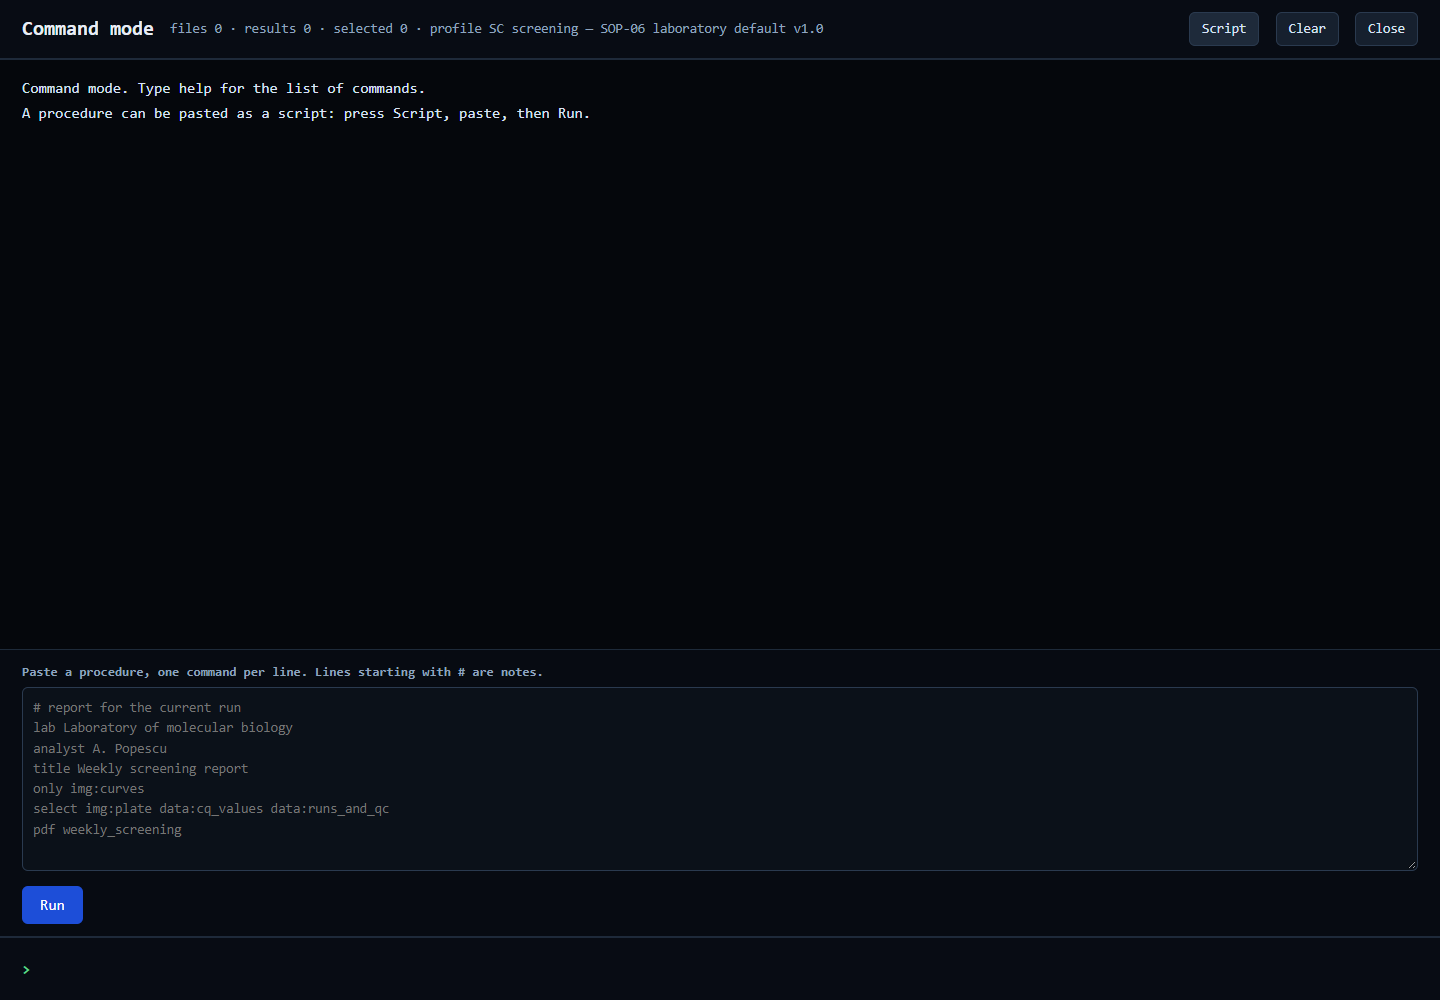
\includegraphics[width=0.98\textwidth]{fig/mode_command.png}
\caption{Command mode with the procedure editor and an executable example.}\label{fig:mode-command}
\end{figure}

\section{Console mode}
Console mode presents one selected item at a time. The top navigation changes scope, the card shows the item state and evidence, and the bottom actions move to the previous or next item, open the source view, or return to the page. Graph items use the same renderers as the Graphs tab. The status line reports readiness, memory and the last draw time.

\begin{lstlisting}[style=vstyle,language=text,numbers=left,firstnumber=1]
1 · Load files     2 · SOP             3 · Results
4 · Control panel  5 · Graphs          6 · Quality & forensic review
7 · Open formats   8 · File integrity
Next · Previous · Open view · Return to the page
\end{lstlisting}

\begin{figure}[htbp]\centering
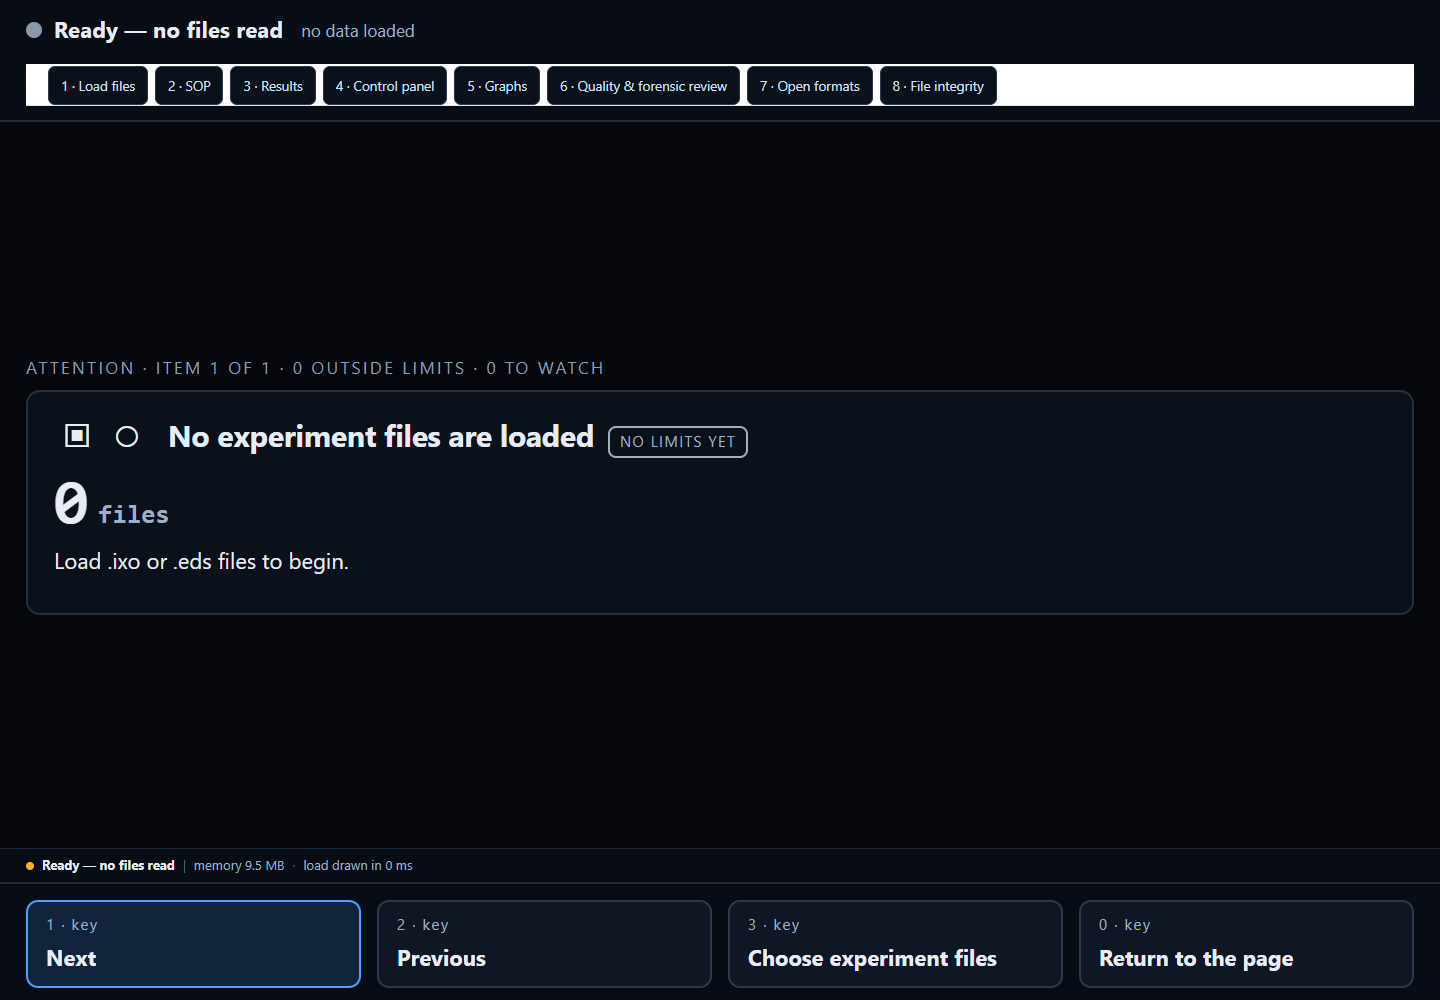
\includegraphics[width=0.98\textwidth]{fig/mode_console.png}
\caption{Console mode in the empty state. The same card becomes a graph or table after data are read.}\label{fig:mode-console}
\end{figure}

\section{Assisted mode}
Assisted mode is a checklist over the catalogue. The operator enters laboratory, analyst and report title, chooses the run for run-level figures, selects PDF, ZIP or both, and checks items by group. The selection can be downloaded as CSV, edited in a spreadsheet and loaded again. Items unavailable for the current data remain visible and explain why.

\begin{lstlisting}[style=vstyle,language=text,numbers=left,firstnumber=1]
# CSV selection example
id,kind,group,title,available,include
img:curves,image,Fluorescence,Amplification curves coloured by SOP outcome,yes,yes
img:plate,image,Plate,Plate heat map,yes,yes
cc:heat_rate,chart,Control charts,Heat rate,yes,yes
data:cq_values,data,Tables,Stored Cq values,yes,yes
\end{lstlisting}

\begin{figure}[htbp]\centering
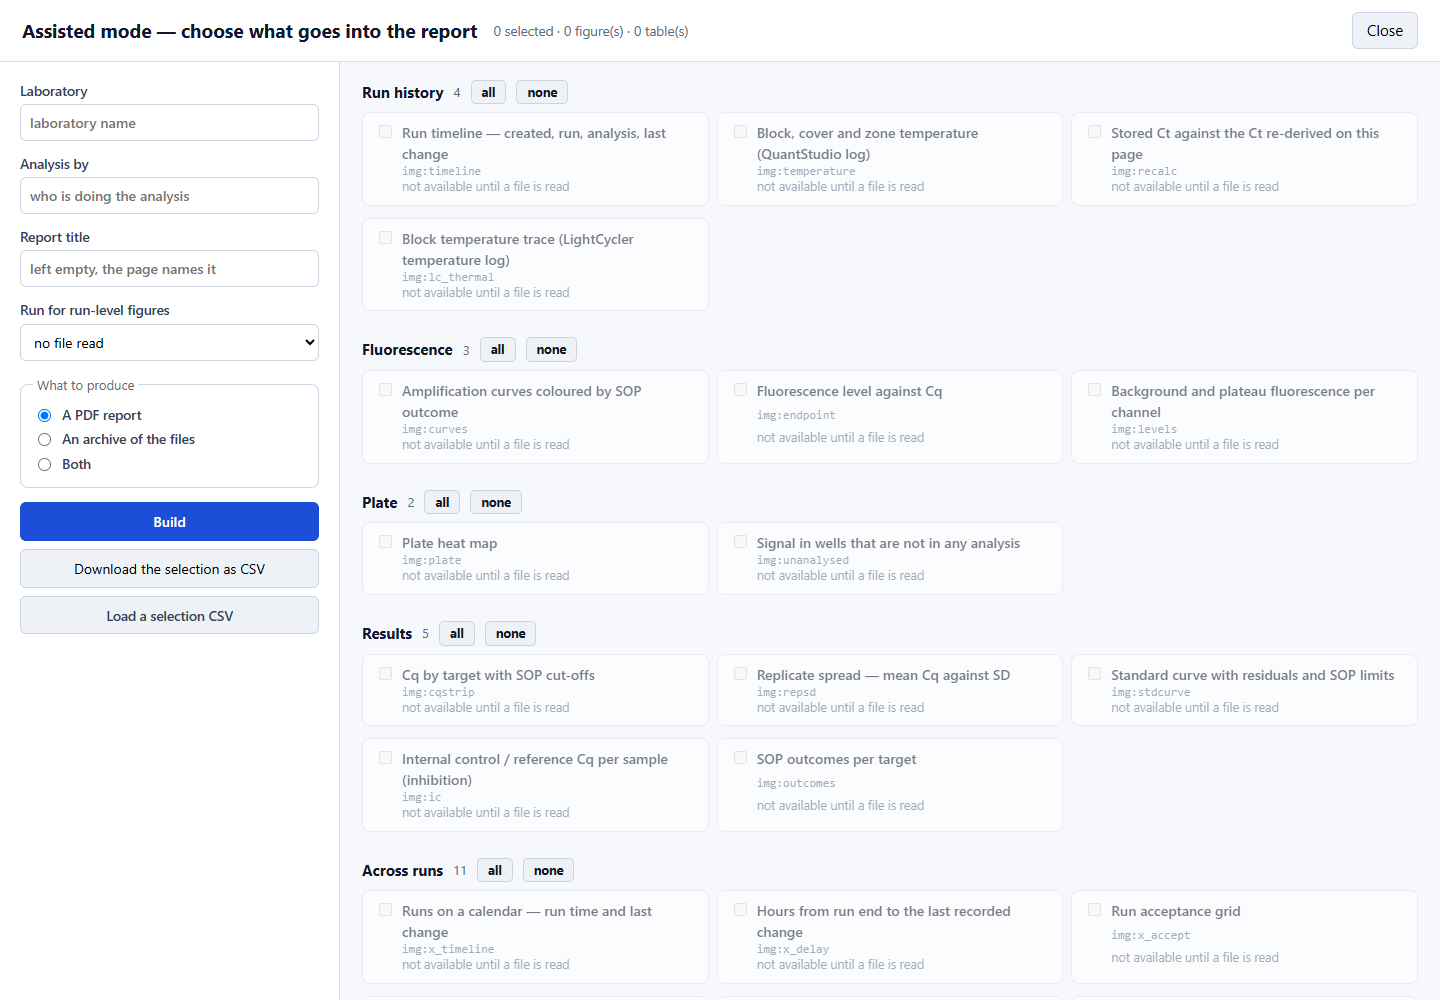
\includegraphics[width=0.98\textwidth]{fig/mode_assisted.png}
\caption{Assisted mode with laboratory metadata, output choice and grouped catalogue checklist.}\label{fig:mode-assisted}
\end{figure}

\section{A procedure}
The box below is the example the page itself offers. Pasting it and pressing Run
produces the same report every week, from whatever files are loaded at the time.

\begin{lstlisting}[style=vstyle,language=text,numbers=left,firstnumber=1]
# report for the current run
lab Laboratory of molecular biology
analyst A. Analyst
title Weekly screening report
only img:curves
select img:plate data:cq_values data:runs_and_qc
pdf weekly_screening
\end{lstlisting}


A multi-line paste into the command line is not run line by line by accident: it
goes to the script box and waits for Run, so a procedure is always read before it
is executed.

\section{Assisted mode}
The same catalogue as a checklist, grouped the way the page groups its figures,
with the laboratory fields, the run the run-level figures use, and the choice of
output. Nothing in it can be done that cannot be done in command mode, and nothing
in command mode is missing from it.

\subsection*{The selection as a file}
A laboratory that always reports the same things should not have to tick the same
boxes. The selection leaves as a CSV and comes back as one. The template carries
every item, whether it is available and whether it is included; only the
\vfn{include} column is read back, so a file written months ago still applies.

{\small
\begin{longtable}{@{}ll@{}}
\toprule \textbf{Column} & \textbf{Meaning} \\\midrule\endfirsthead
\toprule \textbf{Column} & \textbf{Meaning} \\\midrule\endhead
\texttt{id} & the item identifier; this is what is matched \\
\texttt{kind} & figure or table \\
\texttt{group} & the group the item belongs to \\
\texttt{title} & what the item is, for a person reading the file \\
\texttt{available} & whether the loaded data can produce it now \\
\texttt{include} & yes or no; the only column read back \\
\bottomrule
\end{longtable}}

\vhead{The first lines of the template}
\begin{lstlisting}[style=vstyle,language=text,numbers=left,firstnumber=1]
id,kind,group,title,available,include
img:timeline,image,Run history,"Run timeline -- created, run, analysis, last change",yes,no
img:curves,image,Fluorescence,Amplification curves coloured by SOP outcome,yes,no
img:plate,image,Plate,Plate heat map,yes,no
\end{lstlisting}


\section{Who did the work}
A report that cannot be attributed is of little use in a laboratory. The profile
therefore carries two more fields, \vfn{lab.name} and \vfn{lab.analyst}. They are
shown on the profile header, they are printed on every report, and they are part
of the profile --- so the profile checksum changes when they change, and a report
made under one analyst cannot be confused with a report made under another.

\section{The report}
The report is built inside the page. There is no library to load and no service to
call, because the page has to work with no network at all. The writer emits the
1.4 form of the format with the two standard text faces, which are never embedded,
and carries each figure as a compressed image, which the format holds natively.

A report has a cover that states the laboratory, the analyst, the profile and its
checksum, the files that were loaded and what was selected, followed by one
section per item.

{\small
\begin{longtable}{@{}ll@{}}
\toprule \textbf{Part} & \textbf{What it holds} \\\midrule\endfirsthead
\toprule \textbf{Part} & \textbf{What it holds} \\\midrule\endhead
cover & laboratory, analyst, profile, checksum, files, contents \\
figure section & the drawing at the width of the text, then the numbers behind it \\
table section & the table, one row per line, with the number of rows not shown \\
every page & the same text block as this document uses \\
\bottomrule
\end{longtable}}


Two rules govern the tables in a report, and they are the rules this document
follows as well: a row is one line, and a column that does not fit is shortened
rather than wrapped. Column widths are allocated by filling from the narrowest
column upwards, so one wide column cannot take the page.

\section{The code}
The writer, the catalogue and the two windows are printed in full in
Chapter~\ref{ch:val-functions} with the record of what each returned. The two
functions that decide what a report looks like are worth reading here.

\vhead{\vfn{selTableBlock}}
\begin{lstlisting}[language=JavaScript,basicstyle=\ttfamily\scriptsize\color{white},numbers=left,firstnumber=11281]
function selTableBlock(doc,rows,note){
  if(!rows||!rows.length){doc.para("No rows.",9.5,false);return;}
  const cols=uniq(rows.flatMap(Object.keys)).slice(0,8);
  const shown=rows.slice(0,SEL_TABLE_ROWS);
  const size=8.5,gap=6;
  const wid=cols.map(c=>{
    let w=pdfWidth(c,size,true);
    shown.forEach(r=>{w=Math.max(w,pdfWidth(String(r[c]==null?"":r[c]),size,false));});
    return w;
  });
  /* Water-filling: a column never takes more than it needs, and a column that needs
     more than its share only gets the room the others did not use. Scaling every column
     by one factor would spend the page on whichever column happens to be widest. */
  let room=doc.width-gap*(cols.length-1);
  const widths=wid.slice();
  if(wid.reduce((a,b)=>a+b,0)>room){
    let left=room,open=cols.map((c,i)=>i);
    for(let pass=0;pass<8&&open.length;pass++){
      const share=left/open.length,done=[];
      open.forEach(i=>{if(wid[i]<=share){widths[i]=wid[i];left-=wid[i];done.push(i);}});
      if(!done.length){open.forEach(i=>{widths[i]=left/open.length;});break;}
      open=open.filter(i=>!done.includes(i));
    }
  }
  const line=(vals,bold)=>{
    doc.room(size*1.5);
    let x=0;
    vals.forEach((v,i)=>{
      doc.text(pdfFit(v,widths[i],size,bold),size,bold,x);
      doc.y+=size*1.32;                      /* stay on the line for the next column */
      x+=widths[i]+gap;
    });
    doc.y-=size*1.5;
  };
  line(cols,true);
  doc.rule();
  shown.forEach(r=>line(cols.map(c=>{
    const v=r[c];
    return typeof v==="number"?String(+v.toPrecision(6)):String(v==null?"":v);
  }),false));
  doc.gap(2);
  const left=rows.length-shown.length;
  doc.para(left>0?`${rows.length} rows in total; the first ${shown.length} are shown. The archive carries all of them.`
                 :`${rows.length} row${rows.length===1?"":"s"}.`,8,false);
  if(note)doc.para(note,8,false);
}
\end{lstlisting}

\vhead{\vfn{selBuildReport}}
\begin{lstlisting}[language=JavaScript,basicstyle=\ttfamily\scriptsize\color{white},numbers=left,firstnumber=11327]
async function selBuildReport(){
  const chosen=selSelected();
  if(!chosen.length)throw new Error("nothing is selected");
  const doc=pdfDoc();
  doc.text(selReportTitle(),20,true);
  doc.gap(4);doc.rule();doc.gap(6);
  const meta=[
    ["Laboratory",sopLabName()||"not stated"],
    ["Analysis by",sopAnalystName()||"not stated"],
    ["Profile",SOP.name+"  v"+SOP.version],
    ["Profile checksum","sha256:"+sopHash()],
    ["Built",new Date().toISOString().replace("T"," ").slice(0,19)+" UTC"],
    ["Runs loaded",RUNS.length?RUNS.map(runName).join(", "):"none"],
    ["Items selected",String(chosen.length)]
  ];
  meta.forEach(([k,v])=>{
    doc.room(14);
    doc.text(k,10,true);doc.y+=13.2;doc.text(v,10,false,120);
  });
  doc.gap(10);doc.rule();doc.gap(4);
  doc.para("Values in this report are the values the instrument software stored. The page recomputes nothing. "
    +"This is not a validated laboratory report and does not replace the laboratory's own record.",9,false);
  doc.gap(8);
  doc.text("Contents",12,true);
  chosen.forEach((x,i)=>{doc.room(12);doc.text((i+1)+".  "+x.title+"   ["+x.id+"]",9.5,false);});

  for(const x of chosen){
    doc.page();
    doc.text(x.title,14,true);
    doc.gap(2);
    if(x.note)doc.para(x.note,9,false);
    doc.gap(4);doc.rule();doc.gap(4);
    if(x.kind==="image"){
      let f=null;
      try{f=x.figure();}catch(e){doc.para("This figure could not be drawn: "+(e&&e.message||e),9.5,false);}
      if(f){
        const jpg=await svgToJpeg(f.svg,2);
        if(jpg){
          const w=doc.width,h=w*jpg.natH/jpg.natW;
          doc.room(h+10);
          doc.image(jpg.bytes,w,h,jpg.w,jpg.h);
        }else doc.para("This figure could not be rasterised in this browser.",9.5,false);
        if(f.rows&&f.rows.length){
          doc.gap(6);doc.text("Numbers behind this figure",11,true);doc.gap(2);
          selTableBlock(doc,f.rows);
        }
      }
    }else{
      let rows=[];
      try{rows=x.rows()||[];}catch(e){doc.para("This table could not be built: "+(e&&e.message||e),9.5,false);}
      selTableBlock(doc,rows);
    }
  }
  const bytes=doc.build();
  SEL_STATE.lastReport={bytes:bytes.length,items:chosen.length,at:new Date().toISOString()};
  return bytes;
}
\end{lstlisting}

